% !TEX program = xelatex
\documentclass[12pt,a4paper]{article}
\usepackage{fontspec}
\IfFontExistsTF{Times New Roman}{\setmainfont{Times New Roman}}{\setmainfont{TeX Gyre Termes}}
\IfFontExistsTF{Arial}{\setsansfont{Arial}}{\setsansfont{TeX Gyre Heros}}
\IfFontExistsTF{Consolas}{\setmonofont{Consolas}[Scale=0.85]}{\setmonofont{Latin Modern Mono}[Scale=0.85]}
\usepackage[english]{babel}
\usepackage[margin=25mm,headheight=15pt]{geometry}
\usepackage{amsmath,amssymb,graphicx,booktabs,longtable,array,tabularx}
\usepackage{xcolor}
\usepackage{listings,float,fancyhdr,xurl,hyperref}
\hypersetup{hypertexnames=false,colorlinks=true,linkcolor=blue!45!black,urlcolor=blue!55!black,citecolor=blue!45!black,
pdftitle={Assignment 2: Synthetic Image Generator},pdfauthor={Nguyễn Vinh Anh Quân}}
\setlength{\parindent}{1.5em}
\setlength{\parskip}{3pt}
\setlength{\emergencystretch}{3em}
\renewcommand{\arraystretch}{1.2}
\definecolor{tablehead}{HTML}{E7EEF6}
\pagestyle{fancy}\fancyhf{}
\fancyhead[L]{\small Computer Graphics -- Assignment 2}
\fancyhead[R]{\small Implementation Report}\fancyfoot[C]{\thepage}
\lstset{basicstyle=\ttfamily\footnotesize,breaklines=true,columns=fullflexible,keepspaces=true,
showstringspaces=false,frame=single,rulecolor=\color{black!20},backgroundcolor=\color{black!2}}
\newcommand{\code}[1]{{\small\nolinkurl{#1}}}
\newcommand{\source}[1]{\par{\raggedright\footnotesize\textit{Implementation evidence:} \code{#1}.\par}}
\newcommand{\capture}[3]{\begin{figure}[htbp]\centering\includegraphics[width=#3\linewidth]{figures/#1}\caption{#2}\end{figure}}

\begin{document}
\begin{titlepage}\centering
{\normalsize\bfseries VIETNAM NATIONAL UNIVERSITY HO CHI MINH CITY\par}
{\normalsize\bfseries HO CHI MINH CITY UNIVERSITY OF TECHNOLOGY\par}
{\small FACULTY OF COMPUTER SCIENCE AND ENGINEERING\par}\vspace{20mm}
{\large\bfseries Computer Graphics -- CO3059\par}\vspace{8mm}
{\Huge\bfseries Assignment 2\par}\vspace{7mm}
{\LARGE Synthetic Image Generator\par}\vspace{3mm}
{\Large Detection, Instance Segmentation and Depth\par}\vspace{9mm}
{\large Implementation and Mathematical Foundations\par}\vspace{14mm}
\begin{tabular}{ll}
\textbf{Instructors:} & Dr. Thanh-Sach LE, MSc Tram Tran\\
\textbf{Semester:} & I, Academic Year 2026--2027\\
\textbf{Report date:} & November 16, 2026
\end{tabular}\par\vspace{10mm}
\begin{tabularx}{0.85\linewidth}{@{}Xr@{}}
\toprule \textbf{Assignment 2 author} & \textbf{Student ID}\\\midrule
Nguyễn Vinh Anh Quân & 2353007\\\bottomrule
\end{tabularx}\vfill
\small Source repository:\par
\url{https://github.com/AtomTNB2202/CO3059-Assignment2-ComputerGraphic}\par\vspace{5mm}
Assignment 1 foundation credited to Bùi Quốc Thái (2353086).\par
Report prepared from the current local Assignment 2 implementation and assignment v1.2.
\end{titlepage}

\pagenumbering{roman}
\begin{abstract}
This report describes a C++17 synthetic dataset generator built on a custom OpenGL 3.3 Core and GLSL rendering pipeline. An interactive editor imports OBJ meshes and configures object transforms, materials, lighting and camera pose. The exporter captures aligned RGB images, exact instance identifiers, visible-instance masks, bounding boxes and numerical camera-forward depth. Detection labels are exported in both COCO JSON and YOLO TXT formats; COCO also provides compressed run-length instance segmentation. Seeded batch generation varies scene properties from a fixed base scene and stores replayable scene files. An export dialog renders a preview in memory, while a dataset viewer opens saved samples and reports numerical depth under the cursor. This report explains the architecture, coordinate conventions, annotation algorithms, user workflow, verification results and implementation limits. The reported examples contain eight images, forty visible-object annotations and four categories. No learning-based depth estimation or black-box dataset generator is used.
\end{abstract}
\tableofcontents\clearpage\pagenumbering{arabic}

\section{Objectives and Requirement Coverage}
Assignment 2 requires configurable multi-object scenes loaded from external OBJ or PLY files, RGB rendering, detection and segmentation labels, aligned depth maps, and a usable dataset export structure. The deliverables are source code with setup instructions and an English report in both LaTeX and PDF form~\cite{assignment}.

The implementation extends the Assignment 1 editor. Its inherited geometry, camera, object selection and material controls provide the scene-editing foundation. The new work is the dataset pipeline, annotation conversion, numerical depth output, batch generation and dataset inspection.

\noindent\noindent\begin{tabularx}{\linewidth}{@{}p{0.31\linewidth}X@{}}
\toprule Requirement & Implemented behavior\\\midrule
Scene design and rendering & External OBJ meshes, multiple categories, translation/rotation/scale, textures, point light and camera controls.\\
Detection labels & Visible bounding boxes and class labels in COCO JSON and normalized YOLO TXT.\\
Instance segmentation & Exact ID PNG, per-instance binary PNG masks and COCO compressed RLE.\\
Depth labels & Float32 NPY arrays aligned with RGB, plus optional grayscale previews.\\
Usability and export & Selectable outputs/destination, preview, batch progress, metadata, replay scenes and saved-dataset viewer.\\
Optional variations & Seeded changes to transforms, materials, textures, camera, lighting and background.\\
\bottomrule
\end{tabularx}

The application supports static dataset samples. Tracking and image captioning are not implemented. No ray-tracing feature is included in the Assignment 2 application.

\section{System Architecture}
\subsection{Components and responsibilities}
\noindent\noindent\begin{tabularx}{\linewidth}{@{}p{0.30\linewidth}X@{}}
\toprule Component & Responsibility\\\midrule
\code{Application} & Owns editor state; coordinates GUI, rendering, single-sample and batch export.\\
\code{Scene}, \code{SceneIO} & Stable instance IDs, categories, transforms, materials, visibility and JSON scene persistence.\\
\code{Camera} & View/projection matrices, orbit/pan/zoom, movement and framing.\\
\code{Renderer} & Shader-driven drawing, offscreen framebuffer capture, RGB/ID/depth readback.\\
\code{Annotation} & Visible areas, bounding boxes, COCO RLE and merging, YOLO class mapping and labels.\\
\code{Depth} & Depth linearization, NPY serialization/deserialization and grayscale conversion.\\
\code{Batch}, \code{DatasetBatch} & Seeded scene variations, iteration, manifests and restoration of editor state.\\
\code{ExportUi}, \code{Preview} & Export choices, actual in-memory previews, progress and viewport visualization.\\
\code{DatasetView}, \code{DatasetUi} & Read saved samples, switch image modes, browse batch indices and inspect depth.\\
\bottomrule
\end{tabularx}

The data flow is:
\begin{center}
\fbox{\parbox{0.91\linewidth}{\centering
OBJ files + textures + scene JSON + user configuration\\$\downarrow$\\
Scene and camera $\rightarrow$ optional seeded variation\\$\downarrow$\\
OpenGL RGB pass + instance-ID/depth pass\\$\downarrow$\\
Top-left-oriented RGB, IDs and depth arrays\\$\downarrow$\\
Bboxes / binary masks / COCO / YOLO / NPY / metadata\\$\downarrow$\\
Saved sample or batch $\rightarrow$ dataset viewer}}
\end{center}

\subsection{Libraries and implementation ownership}
GLFW 3.4 supplies the window, context and input; GLAD loads OpenGL functions; GLM 1.0.1 supplies vector/matrix operations. Dear ImGui 1.91.9b and ImGuizmo implement the editor widgets and manipulation handles. tinyobjloader 2.0.0rc13 parses and triangulates OBJ files; stb decodes textures and writes PNG files; nlohmann/json 3.11.3 parses/writes JSON. Version pins and archive hashes are declared in CMake.

The project implements framebuffer management, drawing passes, ID encoding, visible bounding boxes, compressed RLE, YOLO conversion, depth linearization/NPY I/O and seeded batch orchestration. Python and pycocotools are optional verification tools, not runtime dependencies. The application does not use Unreal Engine, a complete dataset generator or a neural network to produce annotations. Library roles and asset provenance are documented in \code{THIRD_PARTY.md}.

\section{Scene Construction and Rendering}
\subsection{Geometry, categories and assets}
Each object has an instance ID identifying that particular object and a category ID/name describing its class. Two cups therefore have different instance IDs but share one category. Category IDs remain distinct from global COCO annotation IDs and zero-based YOLO indices.

The main demonstration scene, \code{assets/scenes/tabletop.json}, loads five OBJ instances: a table, two cups, a book and a ball. These form four categories. The assets are simple procedural demonstration models authored by the supplied asset-generation script, not scanned objects. The teacher-provided tetrahedron, teapot, Suzanne and Stanford Bunny are also available in \code{assets/models/basicdemo/} for manual import; their original credits are preserved. These additional models are not automatically inserted into the tabletop scene.

The OBJ importer triangulates faces, generates missing face normals, and supplies planar UV coordinates when texture coordinates are absent. It centers the mesh and fits its largest extent into a two-unit box. Consequently, depth and object dimensions are in scene units rather than the original asset's physical units. OBJ material libraries are not imported; the inspector assigns materials and textures.
\source{src/graphics/ModelImport.cpp; assets/models/basicdemo/CREDITS.txt}

\subsection{Transform and camera pipeline}
Objects store translation, Euler rotation and scale. The model matrix and vertex pipeline are
\begin{equation}
M=T R_z R_y R_x S,\qquad p_{\mathrm{clip}}=PVMp_{\mathrm{local}}.
\end{equation}
GLM constructs these matrices on the CPU; GLSL uses them to transform vertices. The inverse transpose of the linear model matrix transforms normals under nonuniform scaling. The camera's view matrix is based on eye, target and up; the projection matrix is perspective. Aspect ratio is computed from the actual capture width and height.

The editor provides camera orbit, pan, zoom, WASD movement and vertical movement with Q/E. A grid indicates spatial scale. Object picking uses an ID-buffer pass; translation arrows and rotation rings manipulate the selected object. New objects appear near the camera target. These controls are inherited from Assignment 1 and are reused when composing dataset scenes.

\subsection{RGB appearance and clean capture}
Materials support uniform color, Gouraud lighting, per-fragment Phong lighting, textured Phong and wireframe display. The light position and background color are configurable. The RGB dataset pass omits the GUI, reference grid, selection outline and gizmos. A screenshot of the editor is therefore different from an exported RGB image.

For annotation capture, surfaces are filled even when the editor material is wireframe. ID capture disables blending, dithering, multisampling and framebuffer sRGB conversion so identifier bytes remain exact. RGB and annotation captures use the same camera, image dimensions and frozen animation time. Capture saves and restores OpenGL state.
\source{src/core/Renderer.cpp: Renderer::captureDataset; shaders/}

\section{Detection and Segmentation Ground Truth}
\subsection{Instance-ID encoding and image orientation}
The annotation pass uses a depth-tested framebuffer and a constant color per object. ID zero denotes background. The three RGB bytes encode an instance ID as
\begin{equation}
\mathrm{ID}=R+256G+65536B.
\end{equation}
The nearest visible surface determines the pixel ID. Hidden objects, the grid and UI are excluded. OpenGL readback initially has a bottom-left origin; RGB, IDs and depth are flipped together to use a top-left origin. All exported masks, bboxes, depth arrays and cursor coordinates follow that convention.

For instance $i$, its visible binary mask is
\begin{equation}
B_i(x,y)=\begin{cases}1&\mathrm{ID}(x,y)=i,\\0&\text{otherwise}.\end{cases}
\end{equation}
The PNG representation stores foreground as 255 and background as zero. The colored segmentation preview hashes instance IDs into stable display colors. Its colors are for visualization; the exact ID image is the authoritative identifier map.

\subsection{Visible bounding boxes and occlusion}
For every instance with visible pixels, the exporter accumulates minimum and maximum pixel coordinates. Its COCO-style box is
\begin{equation}
[x_{\min},y_{\min},w,h],\quad
w=x_{\max}-x_{\min}+1,\quad h=y_{\max}-y_{\min}+1.
\end{equation}
The inclusive extent preserves one-pixel objects. For example, columns 10--14 and rows 20--22 produce \code{[10,20,5,3]}. The visible area is the number of foreground pixels, not box area. Image boundaries clip the label naturally because only captured pixels are scanned. Disconnected visible regions belonging to one object share one enclosing box.

The annotations describe visible (modal) geometry, not hidden/amodal extents. A fully occluded object has no annotation row or binary mask, but its instance metadata remains available with zero visible pixels and a null bbox. An object outside the image is handled the same way. Depth testing resolves occlusion; no learned segmentation is involved.

\subsection{COCO export}
Each sample has one \code{annotations.json} with \code{images}, \code{categories} and \code{annotations}. Annotation records contain category references, visible bbox, visible area, instance ID and compressed run-length segmentation. The binary mask is traversed in column-major order for COCO compatibility. Runs begin with background; the compressed character representation follows the COCO reference convention~\cite{coco}.

Batch merging assigns distinct image and annotation IDs across samples while retaining stable categories. Images reference the corresponding sample RGB file. Categories are validated for consistent IDs and names. The encoder is implemented in C++; official pycocotools is used only to independently decode and compare outputs during verification.
\source{src/scene/Annotation.cpp: makeCoco; appendCocoSample}

\subsection{YOLO detection export}
YOLO output contains paired PNG images and TXT labels. Each visible object contributes one line:
\begin{lstlisting}
class_index x_center y_center width height
\end{lstlisting}
For an image of width $W$ and height $H$, conversion is
\begin{equation}
x_c=\frac{x_{\min}+w/2}{W},\quad y_c=\frac{y_{\min}+h/2}{H},\quad
w_n=\frac{w}{W},\quad h_n=\frac{h}{H}.
\end{equation}
Coordinates are normalized to $[0,1]$. Original category IDs are sorted and mapped to contiguous class indices beginning at zero, including categories not visible in a particular image. Thus occlusion does not change class numbering between samples. An empty image receives an empty label file. The format follows the Ultralytics detection convention~\cite{yolo}.

\code{classes.json} records the mapping to original category IDs/names; \code{dataset.yaml} records the image path and class names. The exporter does not create a train/validation split: \code{val} is null and must be configured using a separate validation set before training. The YAML contains an absolute final output path; update it if moving the dataset. YOLO output is for detection. Segmentation remains available through COCO RLE and PNG masks.
\source{src/scene/Annotation.cpp: yoloLabels; writeYolo}

\section{Numerical Depth Generation}
\subsection{Depth definition and inverse projection}
The renderer reads the depth buffer as floating-point values $d\in[0,1]$. Perspective depth is nonlinear, so saving those values directly would not produce camera-space depth. Using near and far distances $n,f$ from the same capture camera, the exporter computes
\begin{equation}
z=\frac{nf}{f-d(f-n)}.
\end{equation}
This yields positive camera-forward depth $z=-z_{\mathrm{view}}$. Background is set to zero using the background instance ID, rather than being treated as a surface at the far plane.

Depth is not Euclidean distance from the camera center. In view coordinates, Euclidean range would instead be $\sqrt{x_{\mathrm{view}}^2+y_{\mathrm{view}}^2+z_{\mathrm{view}}^2}$. The current implementation exports axial depth and records this convention explicitly in metadata. Values use scene units; they are not automatically meters.

\subsection{NPY representation and preview}
\code{depth.npy} uses NPY 1.0 with little-endian IEEE float32 dtype \code{<f4}, row-major order and shape \code{[height,width]}~\cite{npy}. Its dimensions and orientation match RGB. Values must be finite and nonnegative. C++ writes the array directly; NumPy is not required for export. The reader used by the dataset viewer supports this exported layout and rejects mismatched dimensions, unsupported headers, invalid values and truncated payloads.

The optional grayscale image uses zero for background and values 1--255 for valid surfaces, with nearer pixels brighter. For a nonconstant valid range,
\begin{equation}
g=1+\operatorname{round}\!\left(254\frac{z_{\max}-z}{z_{\max}-z_{\min}}\right).
\end{equation}
Constant valid depth maps to 255. Min/max normalization is per sample, so grayscale values cannot be compared as physical distances between images. Numerical comparisons must use the NPY array.

\subsection{Depth inspection in the application}
Hovering an image in the export preview or dataset viewer shows pixel coordinates and numerical depth. The viewport also supports this in \textbf{Inspector $>$ Scene view $>$ Depth}. Background is explicitly reported as no surface. The export preview and saved-dataset viewer use export resolution; the live viewport preview limits its longer edge to 1024 pixels to control readback cost. A saved depth PNG without NPY supports visual inspection but cannot provide numerical depth.
\source{src/scene/Depth.cpp; src/gui/DatasetUi.cpp: depthReadout}

\section{Seeded Batch Generation and Dataset Structure}
\subsection{Variations and reproducibility}
Each sample begins from a copy of the base scene. A seed sequence combining the user seed and sample index initializes a Mersenne Twister generator. Transform changes therefore do not accumulate from one sample to the next. Supported variations include horizontal position, Y rotation, scale, material color/mode, texture selection, camera yaw/pitch/distance, point-light position and background color. Objects can have transform variation disabled individually; the tabletop support object can remain fixed.

Batch limits are 1--1000 samples, seed 0--1,000,000 and dimensions 1--2048 pixels per axis. The example config requests eight $640\times480$ samples with seed 42. The current animation time is frozen for a batch. The editor's scene, camera and rendering state are restored afterward, including when an exception or cancellation interrupts generation.

Reproducibility assumes the same source assets, application build, settings and graphics environment. Different GPU/driver rasterization may affect pixels. Exact scene poses and camera settings are saved for replay; the project does not claim universal bit-identical cross-platform rendering. Randomization does not enforce collision-free layouts, minimum visibility or guaranteed object inclusion in the frame.
\source{src/scene/Batch.cpp; src/core/DatasetBatch.cpp}

\subsection{Full-output layout}
\begin{lstlisting}
batch_<timestamp>/
  dataset.json              # batch index and settings
  settings.json             # generation configuration
  base_scene.json           # original scene
  annotations.json          # merged COCO
  yolo/
    dataset.yaml
    classes.json
    images/sample_000001.png
    labels/sample_000001.txt
  sample_000001/
    rgb.png
    instance_ids.png
    instance_preview.png
    mask_<instance_id>.png
    depth.npy
    depth_preview.png
    bbox_preview.png
    annotations.json
    sample.json
    scene.json
    yolo/                   # standalone sample YOLO output
  sample_000002/ ...
\end{lstlisting}

\code{sample.json} records resolution, origin, instance/category IDs, visible areas, bboxes, transforms, materials, source asset paths, camera pose/FOV, lighting and depth conventions. \code{scene.json} is a replayable scene. The batch manifest links sample metadata and image files. Output choices omitted in the dialog have null references rather than misleading paths.

Every export uses a new output folder and rejects an existing destination. Files are written beneath a \code{.partial} directory before a final rename. Failed or canceled work retains that suffix so it is distinguishable from completed data. Metadata and replay scenes are always included; COCO and YOLO require RGB. Optional PNG previews can be omitted independently of the in-memory export preview.

\section{Setup and User Instructions}
\subsection{Build and launch}
Use Windows 10/11, an OpenGL 3.3-capable driver and Visual Studio 2022 or 2026 with Desktop development with C++, Windows SDK and C++ CMake tools. The first CMake configuration needs network access to download pinned dependencies. VS Code is an editor and still needs this compiler toolchain.

From the project root:
\begin{lstlisting}
powershell -NoProfile -ExecutionPolicy Bypass -File scripts/build.ps1 -Run
powershell -NoProfile -ExecutionPolicy Bypass -File scripts/build.ps1 -Test
\end{lstlisting}
The Visual Studio 2026 executable remains \code{out/build/vs18/Debug/ComputerGraphicsAssignment1.exe}; the historical target name is retained for compatibility. Visual Studio 2022 uses \code{vs17}. CMake copies shaders and assets beside the executable. Keep these directories with the program when moving a build.

\subsection{Compose and export a scene}
\begin{enumerate}
\item Open \code{assets/scenes/tabletop.json} using \textbf{Open scene}, or import a model through \textbf{Import OBJ $>$ Browse OBJ... $>$ Import model}.
\item Select objects through the scene list or viewport. Change transform, material, texture, category ID/name and visibility in the inspector. Use Move/Rotate handles for direct manipulation.
\item Set camera and light. \textbf{Focus selected} frames an object. Ensure labels use consistent category names and IDs.
\item Click \textbf{Export...}. Select Current scene or Batch, destination and outputs. For batch settings, use \textbf{Scene $>$ Batch generation}; \textbf{Generate batch...} opens the same export dialog.
\item Inspect RGB, Depth, Segmentation or Bounding boxes in the preview. It is rendered directly in memory and writes no files. For a batch, choose the preview sample index; \textbf{Refresh preview} recaptures it.
\item Click \textbf{Export}. Progress and cancellation are available for batch work. On success, use \textbf{View dataset}, \textbf{Open folder} or \textbf{Open first image}.
\end{enumerate}

\capture{export-dialog.png}{Actual application capture: destination and output selection, including YOLO, with the RGB preview rendered before export.}{1}

\subsection{Browse saved output and replay}
Click \textbf{Dataset... $>$ Open dataset folder...} and choose a folder containing \code{dataset.json} for a batch or \code{sample.json} for one sample. Previous/Next and the Sample slider select records; View switches among RGB, Depth, Segmentation and Bounding boxes. Hover the image for numerical depth if NPY was saved. Missing output modes are reported as unavailable. The viewer reads disk output and does not modify the editor scene. It understands this application's manifests, not arbitrary third-party COCO/YOLO layouts.

To edit or rerender a sample, open its \code{scene.json}. Replay files reference external assets; keep models/textures available. The inspector's \textbf{Scene view} selector separately controls live viewport visualization. Return to Scene/edit to pick objects and manipulate gizmos.

\subsection{Command-line export and common errors}
\begin{lstlisting}
.\out\build\vs18\Debug\ComputerGraphicsAssignment1.exe --export-scene assets/scenes/tabletop.json output/single_new
.\out\build\vs18\Debug\ComputerGraphicsAssignment1.exe --export-batch assets/scenes/tabletop.json output/batch_new assets/configs/batch_demo.json
\end{lstlisting}
The target output directory must not already exist. Missing asset errors require restoring the referenced model/texture or choosing a valid replacement. CMake/compiler errors usually require the Visual Studio C++ workload and SDK. Shader errors require keeping \code{shaders/} beside the executable. Configure/build the entire CMake project rather than running a single source file through Code Runner.

\section{Results and Verification}
\subsection{Rendered dataset examples}
Figure~\ref{fig:outputs} shows aligned outputs from the same captured tabletop sample. Masks and boxes describe visible geometry. Background is black in segmentation and depth previews. The segmentation colors identify instances, including the two cups separately.
\begin{figure}[htbp]\centering
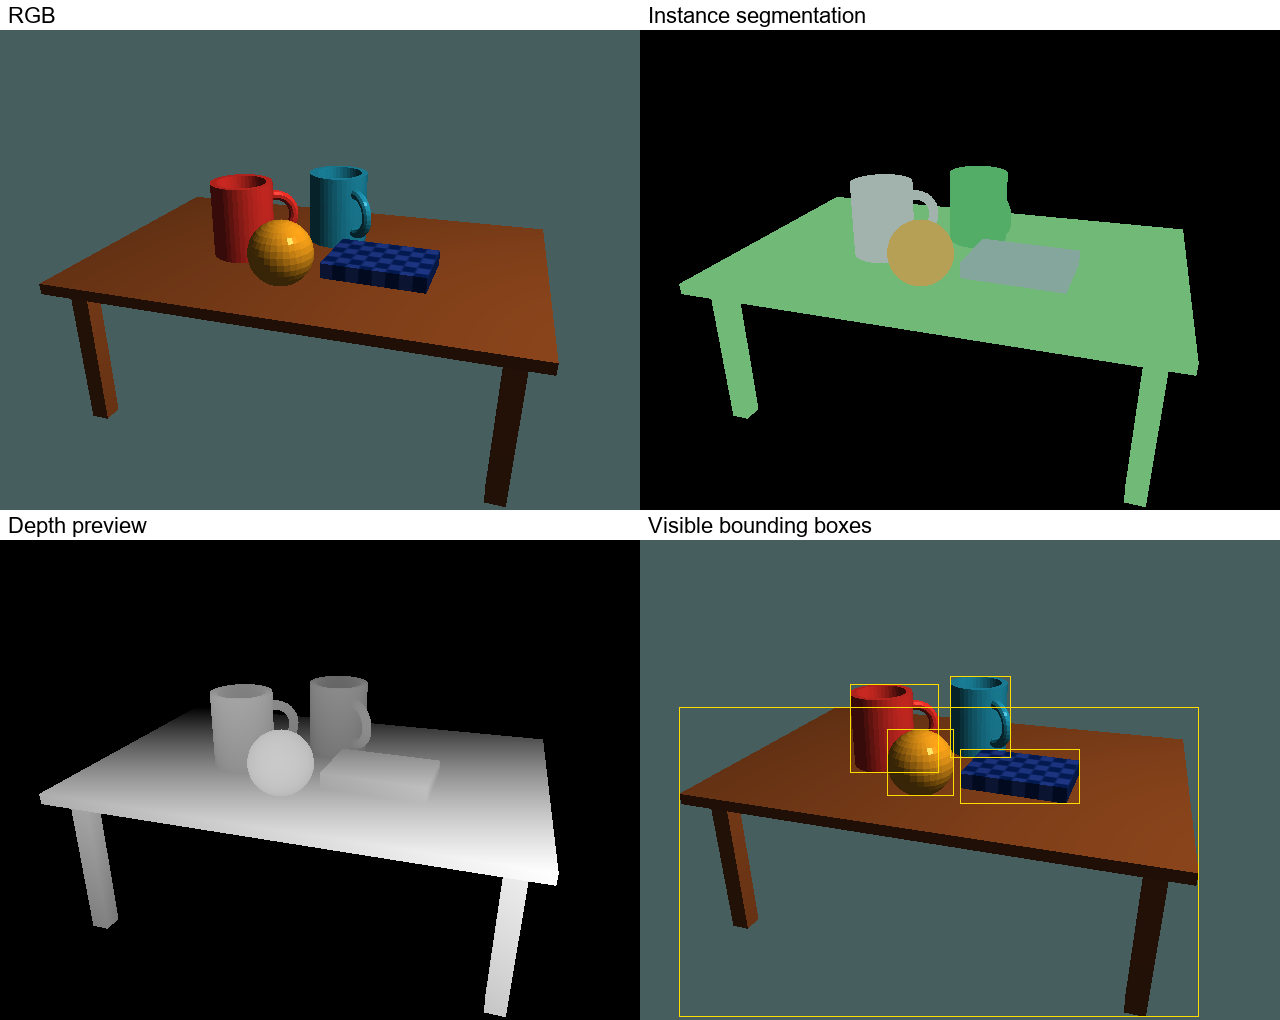
\includegraphics[width=\linewidth]{figures/aligned-outputs.png}
\caption{One $640\times480$ sample: RGB, instance segmentation, depth preview and visible bounding boxes. These are actual C++ exporter outputs, assembled into a panel for the report.}\label{fig:outputs}
\end{figure}

\capture{batch-scenes.png}{All eight RGB samples in the seed-42 demonstration batch. Transform, appearance, camera, light and background variations start from the same tabletop scene.}{1}

\subsection{Automated verification}
On November 16, 2026, CTest completed with all three tests passing: annotations, geometry and graphics smoke. The environment used Windows, Visual Studio 2026 Debug, an NVIDIA GeForce RTX 4070 Laptop GPU and OpenGL 3.3. These checks exercise annotation edge cases, geometry, camera/editor behavior and actual GPU capture/export. The latest run is recorded in \code{report/test-results.txt}.

\noindent\noindent\begin{tabularx}{\linewidth}{@{}p{0.27\linewidth}X@{}}
\toprule Check & Observed result / scope\\\midrule
Annotation unit tests & Visible bboxes/areas; one-pixel and empty masks; COCO RLE fixtures; merge references; normalized YOLO coordinates and sparse-category mapping.\\
Geometry tests & Existing procedural shapes, transforms and the original pyramid OBJ fixture. These are not a visual-quality benchmark.\\
Graphics smoke & Actual OpenGL rendering, editor operations, export dialog preview, batch export and saved-dataset viewer loading.\\
Saved-output round trip & Reopened RGB, instance IDs and float32 depth matched captured arrays; four saved-view modes matched the preview conversion.\\
Independent batch inspection & Eight images, forty boxes, four stable classes; YOLO coordinates agreed with bboxes recomputed from ID pixels; NumPy depth had correct shape/dtype/background; YAML paths referred to final folders.\\
\bottomrule
\end{tabularx}

The independent check uses Pillow and NumPy to read files rather than the C++ viewer. The official pycocotools verification script is also supplied for decoding COCO masks and comparing bbox/area with PNG masks. Tests do not establish performance on every machine, dataset quality for training, or complete coverage of manual GUI interactions. No training-accuracy result is claimed.

\subsection{Inherited scenes}
The source retains the Assignment 1 shape, surface and atom/molecule editor. Figure~\ref{fig:inherited} documents representative inherited scenes for context; they are not new Assignment 2 dataset-generation contributions.
\begin{figure}[htbp]\centering
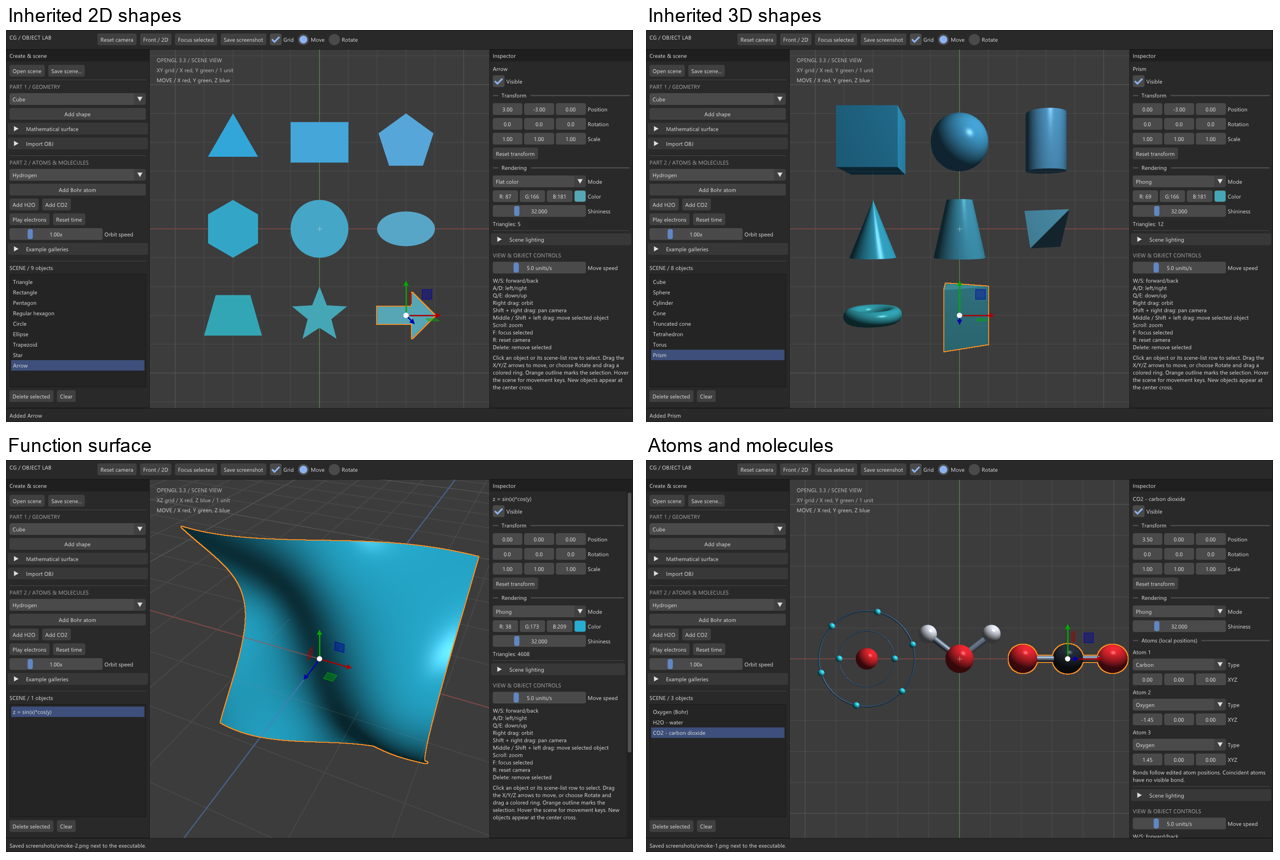
\includegraphics[width=\linewidth]{figures/inherited-scenes.png}
\caption{Supplied Assignment 1 captures: 3D shapes, 2D shapes, sampled surface and atoms/molecules. Original screenshot provenance is retained.}\label{fig:inherited}
\end{figure}

\section{Limitations and Future Work}
The implementation produces aligned ground truth for its own opaque scene rendering, but the following limits affect its use:
\begin{itemize}
\item Visual realism is limited by simple models, a single point light and basic materials. Physically based shading, cast shadows, transparency and ray tracing are absent.
\item Bboxes and masks are visible/modal labels. Fully hidden geometry is not recovered as an amodal annotation.
\item Depth is axial camera-space Z in normalized scene units. It does not include sensor noise or calibrated physical scale.
\item OBJ import is supported; PLY and OBJ material-library import are absent. Missing UVs receive a planar fallback that can distort textures.
\item Random scene variations do not guarantee collision-free placement, a minimum visible area or that all objects remain in the frame. Such constraints would require rejection/resampling rules.
\item YOLO labels are detection boxes. The YAML is a configuration template; a separate validation split and path adjustment after relocation remain user responsibilities.
\item Batch samples are static. Tracking, temporal motion and caption generation are not implemented.
\item The saved-dataset viewer targets the application's own manifest schema. Scene replay depends on availability of referenced assets.
\end{itemize}
Useful future improvements include placement/visibility constraints, more realistic source assets, configurable camera calibration, portable dataset paths and explicit train/validation splitting. These are proposals, not implemented features.

\section{Conclusion}
The application extends a Modern OpenGL editor into a synthetic dataset generator with aligned RGB, detection, instance segmentation and numerical depth output. GPU visibility provides a common basis for IDs, masks and depth, while C++ annotation routines derive COCO and YOLO labels from those visible pixels. Seeded batch generation and replay metadata make experiments inspectable and repeatable within the stated environment. Export previews, depth readout and the saved-dataset viewer allow users to examine results directly in the application. Verification covers the output format, pixel alignment, category consistency and saved-data round trips; the report states the limits of scene realism and dataset generation explicitly.

\clearpage
\phantomsection\addcontentsline{toc}{section}{References}
\begin{thebibliography}{9}
\bibitem{assignment} HCMUT, Department of Computer Science. \textit{Assignments -- Computer Graphics, Semester I, Academic Year 2026--2027}, v1.2. Supplied \code{cgAssignment2.pdf}, cover dated October 27, 2026, Sections 2--3.
\bibitem{project} \textit{CO3059 Assignment 2 source project}. Current local implementation inspected November 16, 2026. Repository: \url{https://github.com/AtomTNB2202/CO3059-Assignment2-ComputerGraphic}. Report describes local changes; it does not assert that every change has already been pushed.
\bibitem{ass1} \textit{Computer Graphics Assignment 1}. Editor foundation and supplied report layout. \url{https://github.com/Funacius/ComputerGraphicsAssignment1}.
\bibitem{coco} COCO API. Compressed mask RLE reference implementation. \url{https://github.com/cocodataset/cocoapi/blob/master/common/maskApi.c}.
\bibitem{yolo} Ultralytics. \textit{Object Detection Datasets Overview}, YOLO label conventions. \url{https://docs.ultralytics.com/datasets/detect/}.
\bibitem{npy} NumPy. \textit{numpy.lib.format: NPY format}. \url{https://numpy.org/doc/stable/reference/generated/numpy.lib.format.html}.
\bibitem{resources} Teacher-provided \code{basicdemo.zip} and \code{cglibs.zip}. Additional OBJ provenance is preserved in \code{assets/models/basicdemo/CREDITS.txt}. Python demo code is not linked into the C++ application.
\end{thebibliography}
\end{document}
